\documentclass{article}




% if you need to pass options to natbib, use, e.g.:
%     \PassOptionsToPackage{numbers, compress}{natbib}
% before loading neurips_2019

% ready for submission
% \usepackage{neurips_2019}

% to compile a preprint version, e.g., for submission to arXiv, add add the
% [preprint] option:
%     \usepackage[preprint]{neurips_2019}

% to compile a camera-ready version, add the [final] option, e.g.:
     \usepackage[final]{neurips_2019}

% to avoid loading the natbib package, add option nonatbib:
%     \usepackage[nonatbib]{neurips_2019}

\usepackage[utf8]{inputenc} % allow utf-8 input
\usepackage[T1]{fontenc}    % use 8-bit T1 fonts
\usepackage{hyperref}       % hyperlinks
\usepackage{url}            % simple URL typesetting
\usepackage{algorithm}% http://ctan.org/pkg/algorithms
\usepackage{algpseudocode}% http://ctan.org/pkg/algorithmicx
\usepackage{tikz}
\usetikzlibrary{shapes.geometric, arrows}

\tikzstyle{io}=[rectangle, minimum width=3cm, minimum height=1cm, text centered, draw=black, fill=blue!30]
\tikzstyle{conv}=[rectangle, minimum width=3cm, minimum height=1cm, text centered, draw=black, fill=orange!30]
\tikzstyle{pool}=[rectangle, minimum width=3cm, minimum height=1cm, text centered, draw=black, fill=green!30]
\tikzstyle{fc}=[rectangle, minimum width=3cm, minimum height=1cm, text centered, draw=black, fill=red!30]

\usepackage{booktabs}       % professional-quality tables
\usepackage{amsfonts}       % blackboard math symbols
\usepackage{nicefrac}       % compact symbols for 1/2, etc.
\usepackage{microtype}      % microtypography
\usepackage{natbib} 
\setlength{\bibsep}{0.0pt}
\title{Robust Convolutional Malware Classification using Defensive Distillation and Feature Squeezing}

% The \author macro works with any number of authors. There are two commands
% used to separate the names and addresses of multiple authors: \And and \AND.
%
% Using \And between authors leaves it to LaTeX to determine where to break the
% lines. Using \AND forces a line break at that point. So, if LaTeX puts 3 of 4
% authors names on the first line, and the last on the second line, try using
% \AND instead of \And before the third author name.

\author{%
   Saranya Vijayakumar\\%\thanks{Use footnote for providing further information
  %   about author (webpage, alternative address)---\emph{not} for acknowledging
  %   funding agencies.} \\
  Computer Science Department\\
  % Carnegie Mellon University\\
  % Pittsburgh, PA 15213 \\
   \texttt{saranyav@cs.cmu.edu} \\
  % examples of more authors
   \And
    Huy Quyen Ngo \\
    Robotics Institute \\
    \texttt{huyquyen@cs.cmu.edu} \\
  % Affiliation \\
  % Address \\
  % \texttt{email} \\
   \AND
   Kriti Kukreja \\
   Information Networking Institute \\
    \texttt{kkukreja@andrew.cmu.edu} \\
  % Affiliation \\
  % Address \\
  % \texttt{email} \\
   \And
   Atharva Mhaskar \\
   Mechanical Engineering Department \\
    \texttt{saranyav@andrew.cmu.edu} \\
  % Address \\
  % \texttt{email} \\
  % \And
  % Coauthor \\
  % Affiliation \\
  % Address \\
  % \texttt{email} \\
}

\begin{document}

\tikzstyle{conv} = [rectangle, minimum width=2cm, minimum height=1cm,text centered, draw=black, fill=blue!30]

\tikzstyle{pool} = [rectangle, minimum width=2cm, minimum height=1cm,text centered, draw=black, fill=red!30]

\tikzstyle{fc} = [rectangle, minimum width=2cm, minimum height=1cm,text centered, draw=black, fill=green!30]
\maketitle

\begin{abstract}
In recent years, the use of computer vision -- specifically through convolutional neural networks -- for malware detection has become increasingly popular. However, it has been discovered that training these models using the malware binaries is highly susceptible to adversarial attacks, which can significantly compromise the effectiveness of the detection process. To mitigate this issue, we propose implementing a combination of defensive distillation and robustness techniques to create a more reliable model for malware classification. We propose using defensive distillation  to create a more abstract representation of the data, which is less vulnerable to adversarial perturbations. The proposed technique also utilizes feature squeezing to compress the input data and remove redundant features, making it more difficult for attackers to manipulate the model's output. This process, combined with defensive distillation, creates a more robust and reliable model for malware classification. By implementing these techniques, we aim to improve the security and accuracy of malware detection models, and better protect against adversarial attacks. By implementing these techniques, we were able to achieve an improvement in classification accuracy by x\%. \end{abstract}

\section{ Introduction }

Convolutional neural networks (CNNs) have demonstrated promising results in anomaly detection, particularly in the field of malware detection. Malware detection using deep learning eliminates the need for standard methods of feature engineering and feature extraction, as raw bytes of executables are fed into the neural network. This approach is more robust to concept drift since features are not engineered by domain experts, making it theoretically better at detecting zero-day malware.

CNNs are particularly suited for malware detection using bytes, as there is structural dependence between adjacent bytes, and CNNs can take advantage of that to study spatial correlations. \citet{raff2017malware} uses deep learning, feeding raw bytes of executables to a neural network, eliminating the need for standard methods of feature engineering and feature extraction. Using the raw bytes of the files would therefore in theory be more robust to concept drift, the idea that malware creators are constantly changing malware to evade detectors, because features are often engineered by domain experts. It should therefore be able to detect zero-days for the same reason.

However, despite the success of CNNs in malware detection, they are vulnerable to adversarial attacks. Adding imperceptible noise to malware images can fool the CNN and lead to misclassification, as shown by previous studies \citep{grosse2017adversarial}.

This presents a serious security risk, as attackers can craft adversarial images to evade malware detectors. To address this challenge, we propose developing a CNN architecture that can accurately classify malware images even in the presence of adversarial noise. Our approach includes investigating various adversarial attack methods and exploring ways to enhance the robustness of the proposed CNN.

%By improving the robustness of malware detection systems, our proposed method has the potential to significantly enhance their reliability and effectiveness in detecting zero-day malware and other advanced threats. Additionally, it can help to prevent attackers from evading detection and causing damage. Our project aims to provide a better understanding of the robustness of CNNs in malware detection, and the potential benefits of enhancing their security in the face of adversarial attacks.

In this project, we aim to address this challenge by developing a CNN architecture that can classify malware images accurately even in the presence of adversarial noise. We will also investigate various adversarial attack methods and explore ways to enhance the robustness of the proposed CNN.

Our proposed method has the potential to significantly improve the reliability and effectiveness of malware detection systems in detecting zero-day malware and other advanced threats. The ability to withstand adversarial attacks can also help to prevent attackers from evading detection and causing damage.


\section{Background}
There has been significant research on using machine learning techniques for malware detection. One approach is to use support vector machines (SVM) to identify behavioral changes within a malware family \citep{wadkar2020detecting}. Another approach is to train models on a dataset of benign PE files and use the entire raw binary as input to detect malicious samples \citep{raff2017malware}. Visual similarity among malware instances can also be used for classification using standard image features \citep{nataraj2011malware}. A combination of convolutions followed by long short-term memory (LSTM) is used to process the sequence of application programming interface (API) calls generated by malware files \citep{kolosnjaji2016adaptive}. \\
Deep learning techniques, such as convolutional neural networks (CNNs), have also been used for malware classification by converting malware samples into grayscale images \citep{hsiao2019malware}. However, these models are not robust to adversarial perturbations, as demonstrated by the success of adversarial examples in evading machine learning models \citep{spencer2022dissecting}. This work spurred an entire field of adversarial robustness for malware detection using the raw bytes, including much work that uses CNNs on the bytes.  Papers like \citet{suciu2019exploring} demonstrate architectural weaknesses of using convolutions on the bytes. 

%\citet{hu2023generating}


\subsection{Using raw bytes as input}

MalConv is a common technique for malware detection that leverages convolutional neural networks (CNNs). This approach utilizes a sliding window method to divide the input file into smaller segments, which are then fed into a 1D CNN. The network is trained on a large dataset of both malicious and benign files, with the aim of distinguishing between the two based on the byte sequence patterns in the input files. By learning to recognize these patterns, MalConv can effectively identify malicious code and aid in the detection of potential threats.


%TODO change wording of below 
MalConv combines an 8-dimensional, learnable embedding layer with a 1-dimensional gated convolution. The embedding ideally puts bytes that have semantically similar behaviors closer together. The convolutional layer iterates over non- overlapping windows of 500 bytes each, with a total of 128 convolutional filters. A global max pooling is applied to the gated outputs of the convolutional layer to select the 128 largest-activation features, without considering the structure or locality of those features within the binary. The corresponding values are then used as input to a fully-connected layer for classification. While the original MalConv model considers a maximum input file size of 2MB, the model used in our experiments is that provided by Anderson et al. [3], trained on the EMBER dataset with a maximum input file size of 1MB. Files exceeding the maximum allowable size are truncated, while shorter files are padded using a special padding token separate from the standard bytes in the file (i.e., resulting in 257 unique tokens).

\begin{figure}
  \centering
  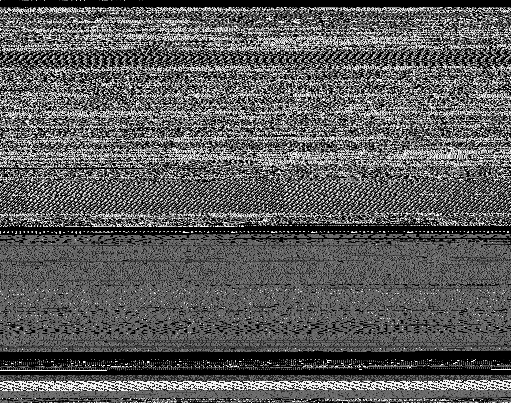
\includegraphics[width=0.7\textwidth]{IMG/Adialer.png}
  \caption{Example of Grayscale Image (Adialer malware sample)}
  \label{fig:adialer}
\end{figure}

In Figure~\ref{fig:adialer}, we see an example of the Adialer malware. 

\subsection{Adversarial attacks}
The Fast Gradient Sign Method (FGSM) is a simple yet effective method to generate adversarial images \cite{goodfellow2014explaining}.

FGSM adds a small perturbation to the input data such that the resulting perturbed data causes the targeted model to misclassify the input data. The perturbation is calculated by taking the gradient of the loss function of the model with respect to the input data and then adding a small value (usually a multiple of the sign of the gradient) to the input data.

More specifically, in the FGSM attack, an attacker computes the gradient of the loss function of the model with respect to the input data, evaluates the sign of the gradient, and then adds a small multiple of the sign of the gradient to the input data to create an adversarial example. The magnitude of the perturbation is typically controlled by a hyperparameter called the epsilon value.

An adversarial attack that modifies a malware sample to evade detection by a classifier can impact the security of a system if the classifier is used as a defense mechanism to protect against malware.

If using a byte-level malware classifier like MalConv to detect and block malware at the network level, an attacker could potentially evade detection by modifying the malware sample using an adversarial attack. This could allow the attacker to bypass the organization's defenses and deliver the modified malware to the target system. However, the modified malware may not be fully functional or may even be non-functional. 

\subsection{Robustness}

Robustness has been an important topic of discussion in this field, especially with the rise of deep learning malware detectors, which are by nature less robust. However, popular papers like \cite{vinayakumar2019robust} make no robustness claims and do not even evaluate against adversarial attacks. 

\citet{demetrio2021adversarial} indicates that we can add protections, including distillation and re-training on adversarially crafted samples. We may also be able to strengthen models against adversarial attacks by including additional structure in the training process.

However, \citet{grosse2016adversarial} showed that feature reduction in particular does not improve robustness. This is at odds with general, non malware-related work that shows pruning does improve adversarial robustness of neural networks. The prior work keeps features with high mutual information, and based on where/how often they appear. We propose to use other, more standard pruning methods to see if this does in fact improve robustness. We will also combine this with defensive distillation:  training a larger neural network to learn a soft target distribution and then using the output of this network as a guide for training a smaller network to improve its robustness. While this has been done for malware, it has not been done for malware bytes, and also has not been done using a CNN. 

%MAL2GCN: A Robust Malware Detection Approach Using Deep Graph Convolutional Networks With Non-Negative Weights 
\cite{kargarnovin2021mal2gcn} (Mal2GCN) proposes a deep learning-based approach for malware detection that employs graph convolutional networks (GCNs) to learn the features of malware graphs and classify them as either benign or malicious. Unlike previous approaches, Mal2GCN utilizes non-negative weights in its GCN architecture to make it more robust to adversarial attacks. However, the method may require more computational resources and GCNs are generally less interpretable compared to CNNs, which may make it more challenging to understand the behavior of the model and diagnose any issues.
%https://ieeexplore.ieee.org/stamp/stamp.jsp?arnumber=8703786

%Adversarial Examples for CNN-Based Malware Detectors 
\cite{chen2019adversarial} explores the vulnerability of CNN-based malware detectors to adversarial attacks. The paper proposes a novel approach for generating adversarial examples that successfully fools the CNN-based malware detectors, resulting in high false negative rates. To mitigate the vulnerability, the paper proposed an ensemble defense mechanism that combines multiple models to improve the accuracy of malware detection in the presence of adversarial examples. However, compared to defensive distillation with CNNs, the ensemble defense mechanism may have some weaknesses such as increased computational complexity, reduced interpretability, and performance that depends on the diversity and quality of the ensemble models. Defensive distillation, on the other hand, is a lightweight and widely applicable approach that has been shown to be effective against various adversarial attacks.

%Generation and Evaluation of Adversarial Examples for Malware Obfuscation 
\cite{park2019generation} discusses the susceptibility of neural networks to adversarial examples, which allow malicious actors to evade classifiers. While small perturbations to input are usually used to create adversarial examples, they are not effective with malware. The paper presents a generative model for executable adversarial malware examples using obfuscation, which achieves a high misclassification rate of up to 100 percent and 98 percent in white-box and black-box settings, respectively. However, compared to defensive distillation with CNN, there are some weaknesses such as reliance on specific obfuscation techniques that may not be effective against more advanced malware detection systems, increased computational complexity of the malware detection system due to the obfuscation techniques used, and dependence on the quality and diversity of the ensemble models used in the defense mechanism. 

%https://ieeexplore.ieee.org/stamp/stamp.jsp arnumber=8999277

%Malware Evasion Attack and Defense 
\cite{huang2019malware} discusses white-box and grey-box evasion attacks to machine learning based malware detector. The JSMA attack proves that a small modification of the feature vector can evade machine learning based malware detector.
%https://ieeexplore.ieee.org/stamp/stamp.jsp?arnumber=8806017

%Adversarial Malware Binaries: Evading Deep Learning for Malware Detection in Executables 
\cite{kolosnjaji2018adversarial} discusses the vulnerability of malware detection by successfully evading state-of-the-art malware detectors while retaining the original functionality of the malware. The paper also proposes a defense mechanism using adversarial training, which improves the robustness of malware detection models against adversarial examples. By training the malware detection model with both clean and adversarial examples, the model becomes more robust to adversarial attacks and can successfully detect the adversarial examples generated by their approach. 
%However, the proposed method only focuses on generating adversarial examples for binary files and does not consider other types of malware, while defensive distillation with CNN can be applied to a wider range of models and data types. The proposed method requires access to the targeted malware detector during the adversarial example generation process, while defensive distillation with CNN does not require this access. Finally, the proposed method relies on adversarial training for defense, which is less effective than defensive distillation with CNN in terms of reducing the model's vulnerability to adversarial attacks.
%https://cs.paperswithcode.com/paper/adversarial-malware-binaries-evading-deep



% Defensive distillation

% Generation & Evaluation of Adversarial Examples for Malware Obfuscation: %https://ieeexplore.ieee.org/abstract/document/8999277/

Adversarial examples for malware detection (grosse, papernot)
This paper uses defensive distillation, but uses the DREBIN dataset, which is feature-extracted data. We will advance the field by uniquely applying robustness methods to raw bytes. 

% Malware evasion attack and defense
% %https://ieeexplore.ieee.org/abstract/document/8806017/

% Adversarial examples for cnn-based malware detectors
% %https://ieeexplore.ieee.org/abstract/document/8703786/


\section{Methods}

We propose to add robustness to convolutional networks used to detect malware. We first obtain the image dataset, Malimg, which is the popular malware image dataset of greyscale images. Then we implement prior work including MalConv to provide ourselves a foundation from which to build our robustness. We then replicate adversarial benchmark models. We create our own method using defensive distillation and feature squeezing. We test this method for precision and recall to see if it improves from the original MalConv against adversarial data. 


More information and some preliminary work can be found on our project's github: \href{https://github.com/svijayakumar2/malware-cv}{https://github.com/svijayakumar2/malware-cv}. 

% We seek to make a network that is as small as possible, for high resolution image analysis. 

% Many typical pruning methods rely on saliency metrics, which are extremely noisy, especially on a network that has not been trained. 
% Instead, a spectral analysis can be used to automatically find a threshold for pruning, without requiring training or evaluation on dataset.  Using the LRP of weights should be a better estimate of performance on the dataset we hope to meet state-of-the-art pruning while improving explainability.

% However, this method of pruning would likely introduce possible adversaries: we aim to test this theory by comparing the robustness of the pruned model versus a typical model. 


\subsection{Dataset}
The Malimg dataset is a collection of malware images, which was created and used in \citet{nataraj2011malware}. The dataset consists of 9,339 grayscale images of size 256x256 pixels, representing 25 different types of malware. Each image has a corresponding label indicating the type of malware it represents.

The malware images were generated using the VirusTotal scanner, which analyzes and classifies malware samples. The images were generated by capturing the screenshots of the VirusTotal scanner's report page for each malware sample. The screenshots were then preprocessed to create the final grayscale images.

The Malimg dataset has been widely used for evaluating the performance of various machine learning algorithms for malware detection and classification. It has also been used for developing techniques for visualizing and analyzing malware images. The dataset is part of the \href{https://pypi.org/project/pt-datasets/}{PyTorch dataset collection} from \citet{agarap2020pytorch}. In Figure~\ref{fig:families}, we see the distribution of samples across the 25 families, and we note the unbalanced distribution.


\begin{figure}
  \centering
  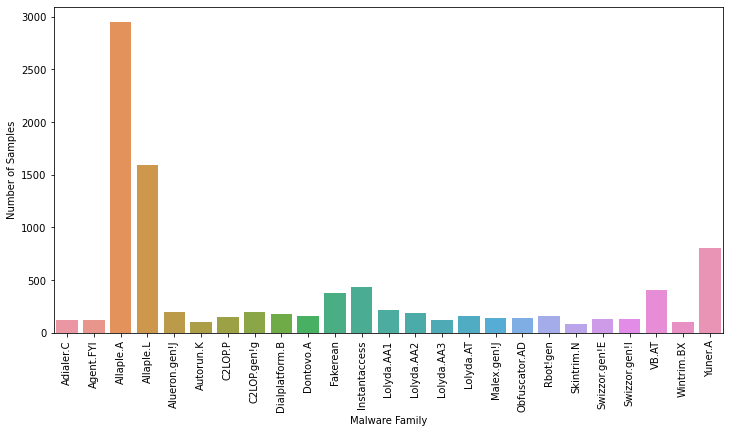
\includegraphics[width=0.7\textwidth]{IMG/families.png}
  \caption{Distribution of Malware Families in Malimg Dataset}
  \label{fig:families}
\end{figure}


\subsection{Baselines}

For our baselines, we use a CNN model trained on raw pixel data, without any additional preprocessing or augmentation. We then adversarially perturb the data. We describe these baselines below. 
%Transfer learning-based approaches where a pre-trained model on a large dataset is fine-tuned on the malware dataset.

%Adversarial training-based approaches where the model is trained with adversarial examples generated from the same dataset. 

[TODO baseline table: precision/recall/accuracy/F1 of our convnet, of malconv, and of adversarially perturbed]


\begin{equation}
Accuracy = \frac{TP + TN}{TP + TN + FP + FN}
\end{equation}

\begin{equation}
Precision = \frac{TP}{TP + FP}
\end{equation}

\begin{equation}
Recall = \frac{TP}{TP + FN}
\end{equation}

\begin{equation}
F1 = \frac{2 \cdot Precision \cdot Recall}{Precision + Recall}
\end{equation}

\subsubsection{Baseline convnet }

The following is our architecture for our CNN that does multiclass classification on the malware images. 

\begin{figure}[ht]
    \centering
    \begin{tikzpicture}[        io/.style={rectangle, draw=black!60, fill=black!5, very thick, minimum size=1cm},        conv/.style={rectangle, draw=black!60, fill=orange!20, very thick, minimum size=1cm},        relu/.style={rectangle, draw=black!60, fill=blue!20, very thick, minimum size=1cm},        pool/.style={rectangle, draw=black!60, fill=green!20, very thick, minimum size=1cm},        fc/.style={rectangle, draw=black!60, fill=red!20, very thick, minimum size=1cm}    ]
        \node (input) [io] {Input};
        \node (conv1) [conv, below of=input] {Conv2d(3, 32)};
        \node (relu1) [relu, below of=conv1] {ReLU};
        \node (pool1) [pool, below of=relu1] {MaxPool2d};
        \node (conv2) [conv, below of=pool1] {Conv2d(32, 64)};
        \node (relu2) [relu, below of=conv2] {ReLU};
        \node (pool2) [pool, below of=relu2] {MaxPool2d};
        \node (flatten) [io, below of=pool2] {Flatten};
        \node (fc1) [fc, below of=flatten] {Linear(64*56*56, 128)};
        \node (relu3) [relu, below of=fc1] {ReLU};
        \node (fc2) [fc, below of=relu3] {Linear(128, num\_classes)};
        \node (output) [io, below of=fc2] {Output};
        
        \draw [->] (input) -- (conv1);
        \draw [->] (conv1) -- (relu1);
        \draw [->] (relu1) -- (pool1);
        \draw [->] (pool1) -- (conv2);
        \draw [->] (conv2) -- (relu2);
        \draw [->] (relu2) -- (pool2);
        \draw [->] (pool2) -- (flatten);
        \draw [->] (flatten) -- (fc1);
        \draw [->] (fc1) -- (relu3);
        \draw [->] (relu3) -- (fc2);
        \draw [->] (fc2) -- (output);
    \end{tikzpicture}
    \caption{Convolutional neural network architecture.}
\end{figure}

\subsubsection{Adversarial Perturbation}
The L2 gradient is defined as the gradient of the L2 distance between the original input $x$ and the adversarial input $x'$, with respect to the input $x$:

$$\nabla_x \left\lVert x - x' \right\rVert_2 = \frac{x - x'}{\left\lVert x - x' \right\rVert_2}$$

where $\left\lVert \cdot \right\rVert_2$ denotes the L2 norm. 

In the context of adversarial attacks, this gradient can be used to compute the direction in which to perturb the input in order to maximize the L2 distance between the original input and the adversarial input while still maintaining the misclassification.


\subsection{Robustness Techniques}

Our methodology aims to improve the robustness of malware image classification. We employ two major techniques to do so: 

\subsubsection{Feature squeezing}
Malware images, like most images, are susceptible to adversarial examples such as images that are perturbed with noise. In our first method, we alter the input samples to make them more difficult to successfully perturb. Feature squeezing is a technique that attempts to detect these adversarial examples. This technique coalesces multiple samples into a single sample, offering fewer opportunities for adversarial examples to work. 
There are a few ways in which feature squeezing can be achieved; but since we are using grayscale images we try spatial smoothing. 

Given an input image $x$ with pixel values $x_i$ scaled to the range $[0, 1]$, we can apply feature squeezing with bit depth $b$ as follows:

First, we scale the pixel values to the range $[0, 2^b - 1]$:

\begin{equation}
\tilde{x}_i = \lfloor x_i \times (2^b - 1) \rfloor
\end{equation}

Next, we quantize the pixel values to the range $[0, 2^b - 1]$:
\begin{equation}
\hat{x}_i = \frac{\tilde{x}_i}{2^b - 1}
\end{equation}

Finally, we use the quantized pixel values as input to the model.

The resulting quantized image $\hat{x}$ is a compressed representation of the original image $x$. This compression can help to remove small variations in the input that are not important for the model's decision, while still preserving the overall structure of the image. By reducing the amount of information in the input, feature squeezing can also make it more difficult for an adversary to find a perturbation that causes the model to misbehave.

Spatial smoothing reduces the input space by “squeezing” out unnecessary input features. We are tasked with doing this without losing too much predictive accuracy. 

\subsubsection{Defensive distillation}

Defensive distillation involves training a model to produce soft labels, which are used to train a second model that learns to produce the same soft labels. This process of "distilling" knowledge from the original model to the second model results in a more robust and generalized model.

The defensive distillation method is based on the paper \cite{papernot2016distillation}. The paper introduces defensive distillation, a mechanism to reduce the effectiveness of adversarial examples on deep neural networks. The implementation uses LeNet and is trained on CIFAR10 dataset. In our version, we trained the same network on the Malimg dataset of grayscale images of size 256x256 of 25 different types of malware, with the hope that the defensive distillation method would work on our data and purpose. 

Let $\theta_1$ and $\theta_2$ be the parameters of the teacher and student models, respectively. The teacher model is trained on a large dataset with a temperature $T$, and the student model is trained on the logits produced by the teacher model, with a higher temperature $T'>T$. Let $D$ be the training data, $y$ be the labels, and $x$ be the input features.

The teacher model's softmax function is given by:
\begin{equation}
\text{softmax}(z_i) = \frac{e^{z_i / T}}{\sum_{j} e^{z_j / T}}
\end{equation}

The student model's softmax function is given by:
\begin{equation}
\text{softmax}(z_i) = \frac{e^{z_i / T'}}{\sum_{j} e^{z_j / T'}}
\end{equation}

The loss function for defensive distillation is given by:

\begin{equation}
L_{DD}(\theta_1, \theta_2; D) = \frac{1}{|D|} \sum_{(x,y) \in D} H(\text{softmax}(z_{\theta_2}(x)), \text{softmax}(z_{\theta_1}(x) / T))
\end{equation}

where $H$ is the cross-entropy loss function. During inference, the student model uses the regular softmax function:
\begin{equation}
\text{softmax}(z_i) = \frac{e^{z_i}}{\sum_{j} e^{z_j}}
\end{equation}
However, the logits produced by the student model are divided by the temperature $T'$ before being passed through the softmax function. Note that the use of a higher temperature during training allows the student model to learn a smoother decision boundary, which makes it more robust to adversarial attacks.



% 


\subsection{Algorithm}

\begin{algorithm}[H]
\caption{Malware Detection with Preprocessing and Adversarial Attacks}\label{alg:malware_detection}
\begin{algorithmic}[1]
\Procedure{MalwareDetection}{bytes, model}
\State $images \gets \textsc{BytesToGrayscale}(bytes)$ \Comment{Convert bytes to grayscale images}
\State $images \gets \textsc{L2GradientAttack}(images)$ \Comment{Perturb images using L2 gradient attack}
\State $images \gets \textsc{FeatureSqueeze}(images)$ \Comment{Apply feature squeezing to images}
\State $model \gets \textsc{DefensiveDistillation}(model, images)$ \Comment{Defensive distillation of model}
\State $predictions \gets \textsc{MalwareCNN}(images, model)$ \Comment{Run Malware CNN on preprocessed images}
\State \textbf{return} $predictions$
\EndProcedure

\Statex

\Procedure{BytesToGrayscale}{bytes}
\State $images \gets \textsc{DecodeBytes}(bytes)$ \Comment{Decode bytes to images}
\State $images \gets \textsc{Grayscale}(images)$ \Comment{Convert images to grayscale}
\State \textbf{return} $images$
\EndProcedure

\Statex

\Procedure{L2GradientAttack}{images}
\State $fmodel \gets \textsc{PyTorchModel}(model, bounds=(-1,1))$ \Comment{Initialize PyTorch model with appropriate bounds}
\State $attack \gets \textsc{L2FastGradientAttack()}$ \Comment{Initialize L2 gradient attack}
\State $epsilons \gets \textsc{Linspace}(0, 50, num=20)$ \Comment{Create range of epsilon values}
\For{$\epsilon$ in $epsilons$}
\State $raw, clipped, is\_adv \gets \textsc{Attack}(fmodel, images, labels, epsilons=\epsilon)$ \Comment{Apply L2 gradient attack}
\EndFor
\State \textbf{return} $clipped$
\EndProcedure

\Statex

\Procedure{FeatureSqueeze}{images}
\State $squeezed\_images \gets []$
\For{$image$ in $images$}
\State $squeezed\_image \gets \frac{\lfloor 2^b * image \rfloor}{2^b - 1}$ \Comment{Squeeze image with bit depth $b$}
\State $squeezed\_images \gets \textsc{Append}(squeezed\_image)$ \Comment{Add squeezed image to list of squeezed images}
\EndFor
\State $squeezed\_images \gets \textsc{Stack}(squeezed\_images)$ \Comment{Stack squeezed images into array}
\State \textbf{return} $squeezed\_images$
\EndProcedure

\Statex

\Procedure{DefensiveDistillation}{model, images}
\State $T \gets \textsc{TemperatureScaling}(model, images)$ \Comment{Compute temperature scaling parameter}
\State $distilled\_model \gets \textsc{Distill}(model, T, images)$ \Comment{Distill model using temperature scaling parameter}
\State \textbf{return} $distilled\_model$
\EndProcedure

\end{algorithmic}
\end{algorithm}

\subsection{Results}

\begin{figure}[h]
  \centering
  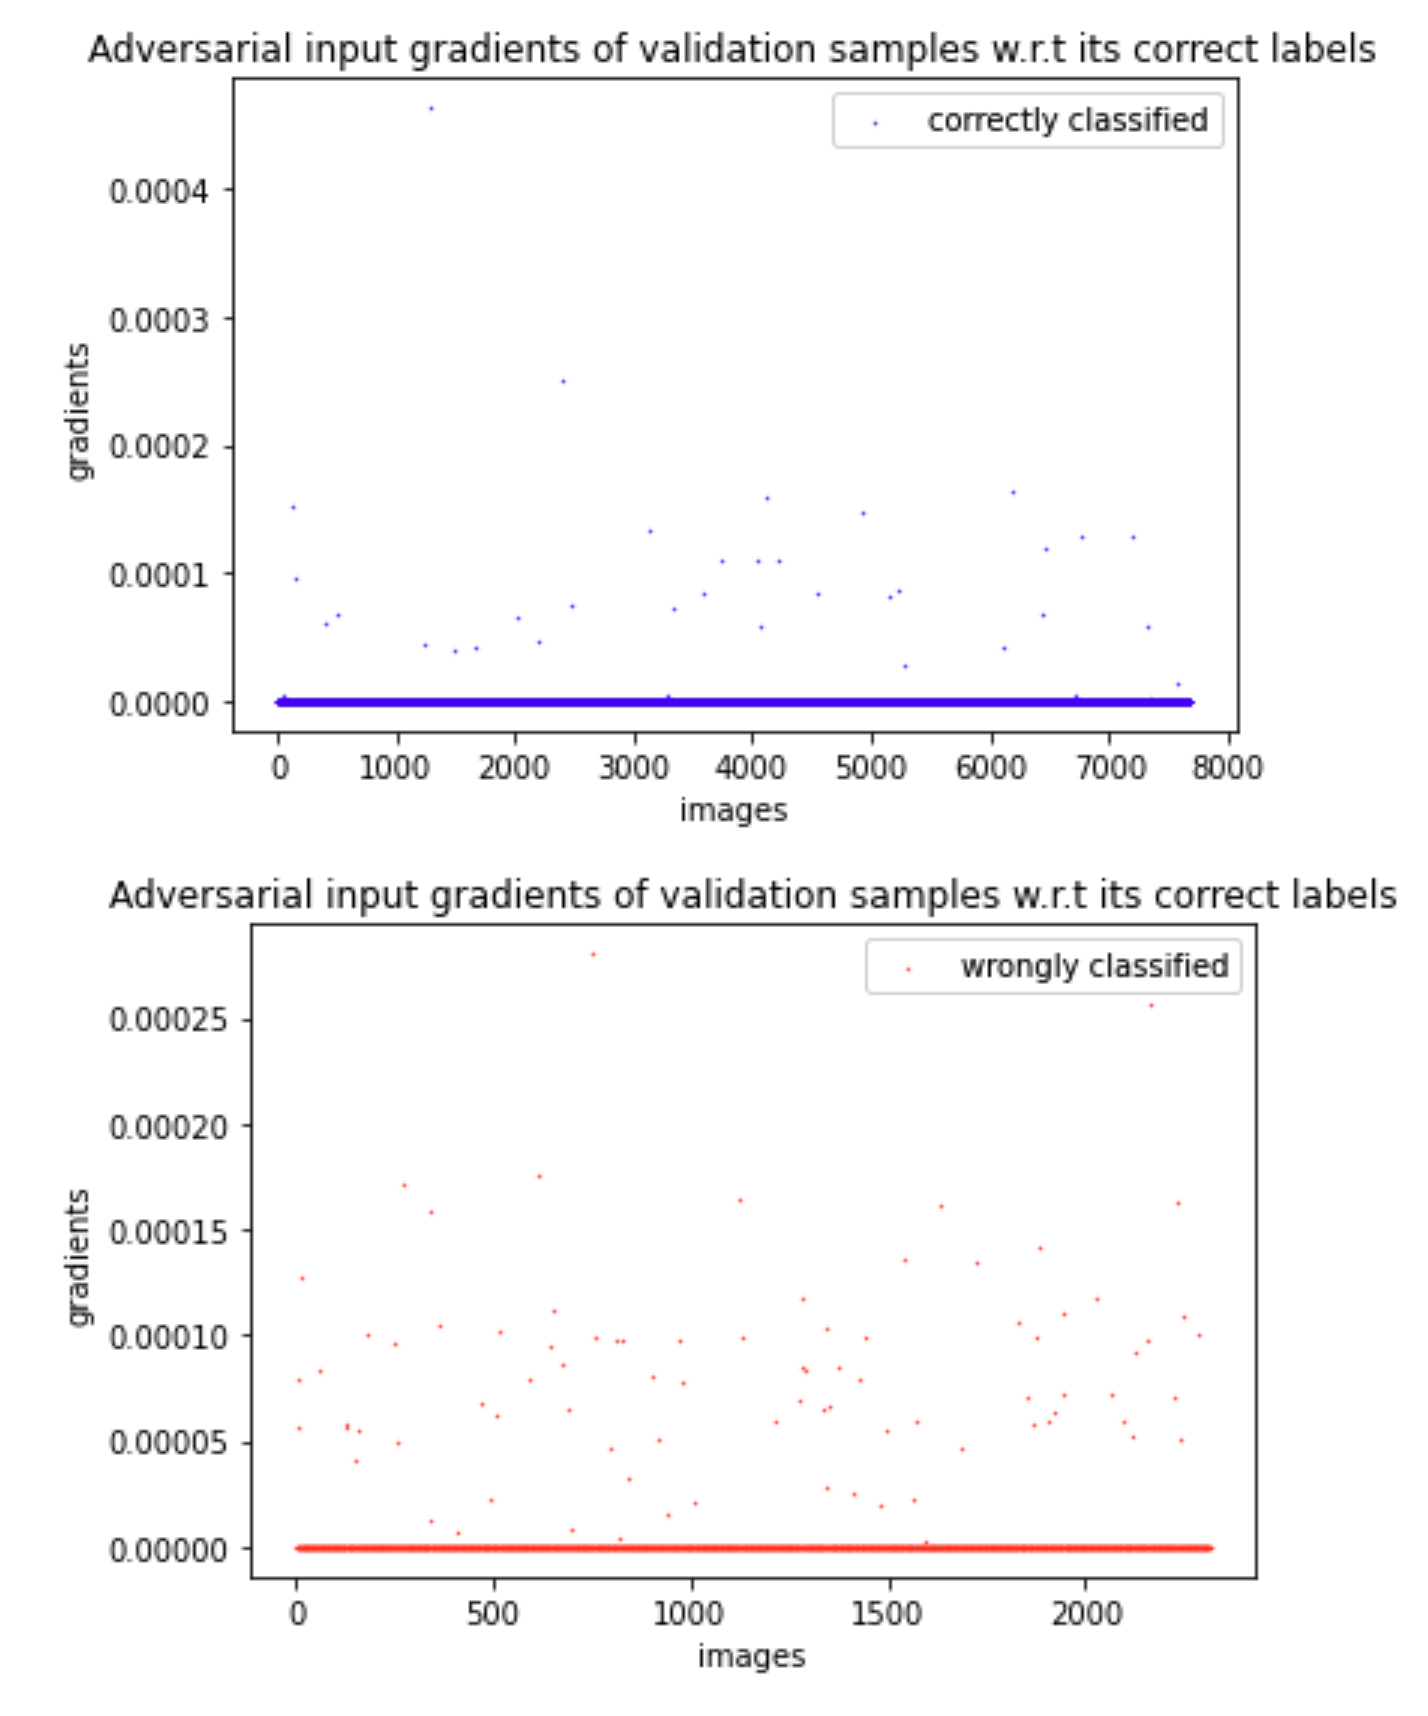
\includegraphics[width=0.7\textwidth]{IMG/Temp-1-distillation.png}
  \caption{Gradient values with temperature = 1}
  \label{fig:temp1-distillation}
\end{figure}


\begin{figure}[h]
  \centering
  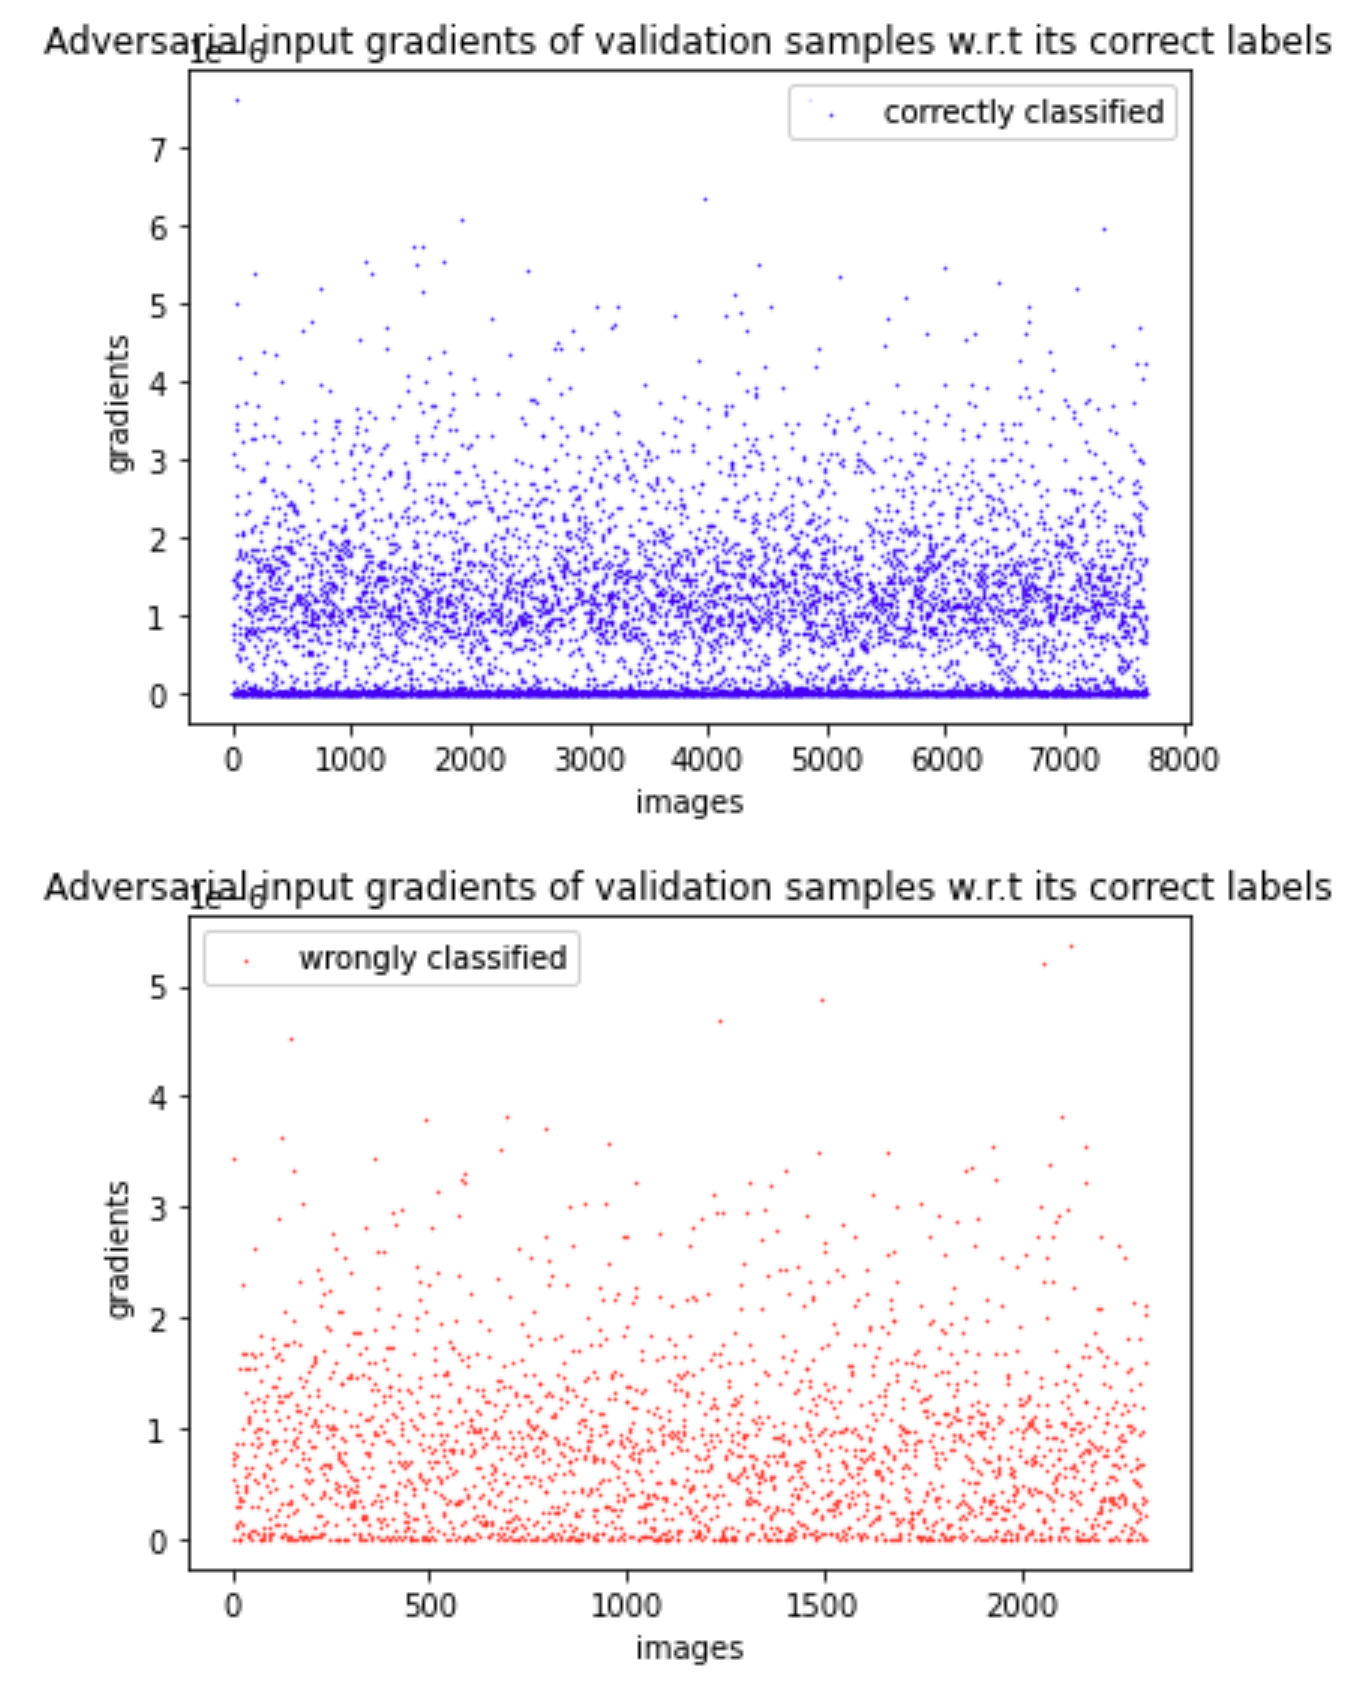
\includegraphics[width=0.7\textwidth]{IMG/Temp-100-distillation.png}
  \caption{Gradient values with temperature = 100}
  \label{fig:temp100-distillation}
\end{figure}

In the implementation on CIFAR10, Figure~\ref{fig:temp1-distillation} and Figure~\ref{fig:temp100-distillation}, varying the temperature hyperparameter in the model changes the effect of distillation in the model. When temperature is 1, the gradient values are very low for correctly classified classes, but very high for misclassified classes, implying that the distillation fails. When the temperature is 100, the gradient norm for misclassified classes are much larger, which is consistent with the fact that losses tend to be large for misclassified classes.


\begin{center}
\begin{tabular}{||c c||} 
 \hline
 Accuracy & Accuracy with Attack \\ [0.5ex] 
 \hline\hline
 95.1 & 12.8  \\ 
 \hline
 \hline
\end{tabular}
\end{center}

{\bf Reproducibility}: we publish our data
and our code, at \url{https://github.com/svijayakumar2/malware-cv}


\small
\bibliographystyle{plainnat}

\bibliography{ref}

\end{document}